\subsubsubsubsection{Crossroads builder}
\begin{figure}[h]
\centering
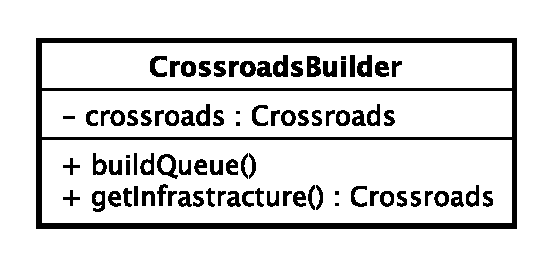
\includegraphics[scale=0.6,keepaspectratio]{images/solution/app/backend/crossroads_builder.eps}
\caption{\pReactiveBuild::CrossroadsBuilder}
\label{fig:sd-app-crossroads_builder}
\end{figure}
\FloatBarrier
\begin{itemize}
  \item \textbf{\descr} \\
    It represents the builder of crossroads entities. 
    \item \textbf{\attrs}
  \begin{itemize}
    \item \texttt{crossroads: Crossroads} \\
The crossroads which the builder incrementally constructs.
  \end{itemize}
  \item \textbf{\ops}
  \begin{itemize} 
    \item[+] \texttt{buildQueue()} \\
Adds a new queue of moving entities to the crossroads.
    \item[+] \texttt{getEntity() : Crossroads} \\
Returns the crossroads.
  \end{itemize}
\end{itemize}
